\documentclass[9pt,twoside,lineno]{pnas-new}
% Use the lineno option to display guide line numbers if required.

\templatetype{pnassupportinginfo}
\usepackage{longtable}

\title{Evolutionary rescue and reintroduction of resistant frogs allows recovery in the presence of a lethal fungal disease}
\author{Roland A. Knapp, Mark Q. Wilber, Allison Q. Byrne, Maxwell B. Joseph, Thomas C. Smith, Andrew P. Rothstein, Robert L. Grasso, Erica Bree Rosenblum}
\correspondingauthor{Corresponding Author name. Roland A. Knapp \\ E-mail: roland.knapp@ucsb.edu}

\begin{document}

\maketitle

%% Adds the main heading for the SI text. Comment out this line if you do not have any supporting information text.
\SItext
\hypertarget{frog-evolution-in-response-to-bd-2}{%
\section{Frog evolution in response to
Bd}\label{frog-evolution-in-response-to-bd-2}}

\hypertarget{methods}{%
\subsection{Methods}\label{methods}}

We compared frog genomes sampled in naive versus recovering populations.
Bd-exposure histories of these populations are based on a decade or more
of data from visual encounter surveys and Bd surveillance using skin
swabbing \citep[e.g.,][]{knapp2016}. Comparing populations with
different infection histories allowed larger sample sizes and
replication across the landscape. The alternative approach of comparing
samples from the same populations before and after Bd exposure isn't
feasible in this system because Bd arrived in most MYL frog populations
decades ago and population persistence/recovery is rare and
unpredictable. As a result, samples from recovering populations
collected from before and after Bd exposure are not available and are
unlikely to be available in the future.

\hypertarget{results-1}{%
\subsection{Results}\label{results-1}}

In the Results section of the main paper, we describe the stringent set
of outlier SNPs (identified using a Bonferroni-corrected p-value of
0.01). The liberal set, identified using a Bonferroni-corrected p-value
of 0.05, included 38 outliers (35 SNPs and 3 INDELS) from 30 distinct
genes across 16 contigs. Our analysis found no significantly
over-represented GO terms in this set of 30 genes, or in the set of 38
outlier regions identified with the splined window analysis.

In the comparison of individual outlier variants between naive and
recovering populations, we detected consistent allele frequency changes
across all genetic clusters for only 1 of 7 of the associated genes
(RIN3; Fig. 1). However, for the other 6
genes we still found a statistically significant signal of selection in
2 of the 3 genetic clusters (containing populations 6--9;
Fig. 1, Figure~\ref{fig-selectionresults}
A). Therefore, although some outlier variant associations have a more
limited geographic extent than RIN3, they still describe parallel
evolutionary changes following Bd exposure and are therefore interesting
candidates for future studies.

\hypertarget{frog-population-recovery-2}{%
\section{Frog population
recovery}\label{frog-population-recovery-2}}

\hypertarget{methods-1}{%
\subsection{Methods}\label{methods-1}}

Swab extracts were analyzed using standard Bd DNA extraction and qPCR
methods \citep{boyle2004}, and extracts were analyzed singly instead of
in triplicate \citep{kriger2006}. For analysis of swabs collected during
2005--2014, we used standards developed from known concentrations of
zoospores \citep{boyle2004}, and after 2014, we used standards based on
single ITS1 PCR amplicons \citep{longo2013}. Based on paired comparisons
between samples analyzed using both types of standards, Bd in the study
area has an average of 60 ITS1 copies per zoospore. To express all qPCR
results as the number of ITS1 copies, starting quantities obtained using
the zoospore standard (measured as ``zoospore equivalents'') were
multiplied by 60. In addition, all qPCR quantities (regardless of
standard) were multiplied by 80 to account for the fact that DNA
extracts from swabs were diluted 80-fold during extraction and PCR
\citep{vredenburg2010}.

\hypertarget{population-viability-modeling-1}{%
\section{Population viability
modeling}\label{population-viability-modeling-1}}

\hypertarget{methods-2}{%
\subsection{Methods}\label{methods-2}}

\hypertarget{incorporating-yearly-variability-in-vital-rates}{%
\subparagraph{Incorporating yearly variability in vital
rates}\label{incorporating-yearly-variability-in-vital-rates}}

We extracted yearly survival probabilities for translocated adults
\(\sigma_{A_T}\) and naturally recruited adults \(\sigma_{A_R}\) from
the CMR model used to estimate population-level parameters of
translocated populations (see ``Materials and Methods - Estimation of
frog survival and abundance'' in main paper). Although we observed
yearly variability in adult survival within a population, the magnitude
of this variability was small compared to among-population variability
(Fig. 3). Thus, we did not include
yearly within-population variability in adult survival in this analysis.
However, within a population there was substantial yearly variability in
the successful recruitment of adults, greater than what we would expect
from Poisson variability around a mean value. Therefore, we allowed for
yearly variability in the probability of successful recruitment
\(\omega\) (additional details provided in ``Estimating model
parameters'' below).

\hypertarget{estimating-model-parameters}{%
\subparagraph{Estimating model
parameters}\label{estimating-model-parameters}}

The baseline parameter values for the model and how they were estimated
are given in Table~\ref{tbl-param_values}. Parameters \(\sigma_{A_T}\)
and \(\sigma_{A_R}\) were extracted directly from our CMR models (see
``Materials and Methods - Estimation of frog survival and abundance'' in
main paper). For populations where we had a sufficient number of
PIT-tagged, naturally-recruited adults, we observed that
\(\sigma_{A_T}\) and \(\sigma_{A_R}\) could be notably different, with
\(\sigma_{A_R} > \sigma_{A_T}\) (Figure~\ref{fig-compare_surv_probs}).
For populations lacking sufficient numbers of naturally-recruited
adults, we were unable to directly estimate \(\sigma_{A_R}\), and
instead set \(\sigma_{A_R} = \sigma_{A_T}\).

\hypertarget{model-analysis-and-simulation}{%
\subparagraph{Model analysis and
simulation}\label{model-analysis-and-simulation}}

We performed four analyses on our model. First, we considered a
deterministic version of our model with no yearly heterogeneity in
probability of successful recruitment \(\omega\), and calculated the
predicted long-run growth rate \(\lambda\) of a population for different
values of \(\sigma_{A_R}\) and \(\omega\). We then fixed
\(\omega = 0.3\) and calculated the predicted growth rate of our 12
populations.

Second, we performed a local elasticity analysis on \(\lambda\) with
respect to parameters \(\omega\), \(\sigma_{A_R}\), and \(F\) to
determine how small changes in these parameters could influence the
long-run deterministic growth rate of populations
(Figure~\ref{fig-viability-supp}).

Third, we defined a version of the model with demographic and
environmental stochasticity, where environmental stochasticity was
represented by among-year variability in \(\omega\). We used this model
to simulate a one-time introduction of 40 translocated adult frogs. We
ran this simulation 1000 times for each population and computed the
probability of a population becoming extinct after 50 years given the
observed parameter values and environmental stochasticity in \(\omega\).
We varied the mean recruitment probability \(\omega\) from 0.15 and 0.4
and drew values of \(\omega\) each year from a beta distribution with a
dispersion parameter of \(\phi = 2\) (when \(\omega = 0.5\) and
\(\phi = 2\) the beta distribution is uniform between 0 and 1).

Finally, we assessed whether our stochastic model could reproduce
observed trajectories of population recovery. We focused on population
70550 because this was our longest CMR time series for a translocated
population and because this population shows evidence of substantial
post-translocation increases in adult abundance associated with
population establishment and recovery. We simulated our model for 16
years, repeating the simulation 50,000 times. For each run and each
year, we drew \(\omega\) from a uniform distribution between 0 and 1 (or
equivalently a beta distribution with mean 0.5 and \(\phi = 2\)). Using
Approximate Bayesian Computing and rejection sampling
\citep{kosmala2016}, we identified the top 2\% of trajectories (i.e.,
1000 trajectories) that minimized the sum of squared errors between the
observed and predicted data. The \(\omega\) values associated with these
``best'' trajectories represented an approximate posterior distribution
\citep{beaumont2010}. Using these best fit trajectories, we assessed
whether our model could qualitatively describe the patterns of recovery
in the observed data for population 70550.

\newpage

\begin{figure}

{\centering 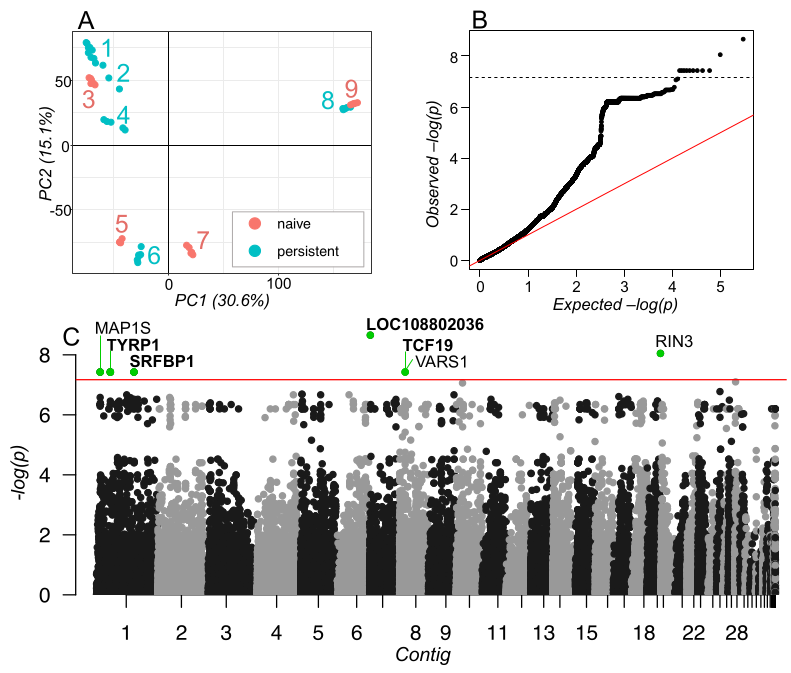
\includegraphics[width=0.85\textwidth]{figures/pca_qq_manhattan.png}

}

\caption{\label{fig-selectionresults}Evidence for selection on
individual variants in recovering MYL frog populations. (A) PCA
calculated from binary SNPs showing the genomic relationship of samples.
Numeric labels and colors match those in
Fig. 1A. Populations 1-7 are \emph{R.
sierrae} and populations 8 and 9 are \emph{R. muscosa}. (B) qqplot
showing observed and expected p-values for 148,307 SNPs and INDELS.
Dashed line shows p-value that identifies outliers. (C) Manhattan plot
showing p-value for each SNP. SNPs are sorted by genomic position and
contigs are sorted by size. Red line shows p-value that identifies
outliers. Outlier SNPs above this threshold are highlighted and labeled.
Bold labels indicate the presence of at least one non-synonymous SNP in
that gene.}

\end{figure}\clearpage

\begin{figure}

{\centering 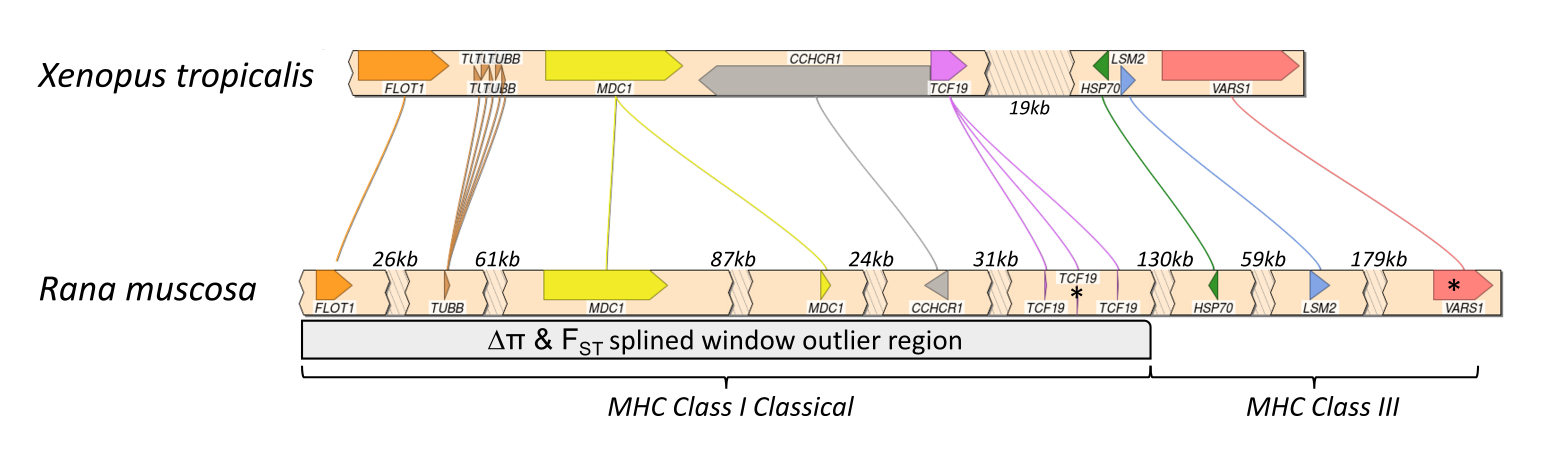
\includegraphics[width=0.85\textwidth]{figures/synteny_figure.png}

}

\caption{\label{fig-synteny-plot}Synteny plot showing conserved gene
order in \emph{Xenopus tropicalis} and \emph{Rana mucosa} for the
outlier region containing MHC Class I Classical and MHC Class III gene
regions. The plot was created with SimpleSynteny \citep{veltri2016}
using \emph{Xenopus tropicalis} Chromosome 8 (NC\_030684.2, genbank
accession GCA\_000004195.4) and \emph{Rana mucosa} Contig19. Asterices
indicate the location of SNP outliers in the TCF19 and VARS1 genes. Gap
sizes for each contig representation are labeled.}

\end{figure}\clearpage

\newpage

\begin{figure}

{\centering 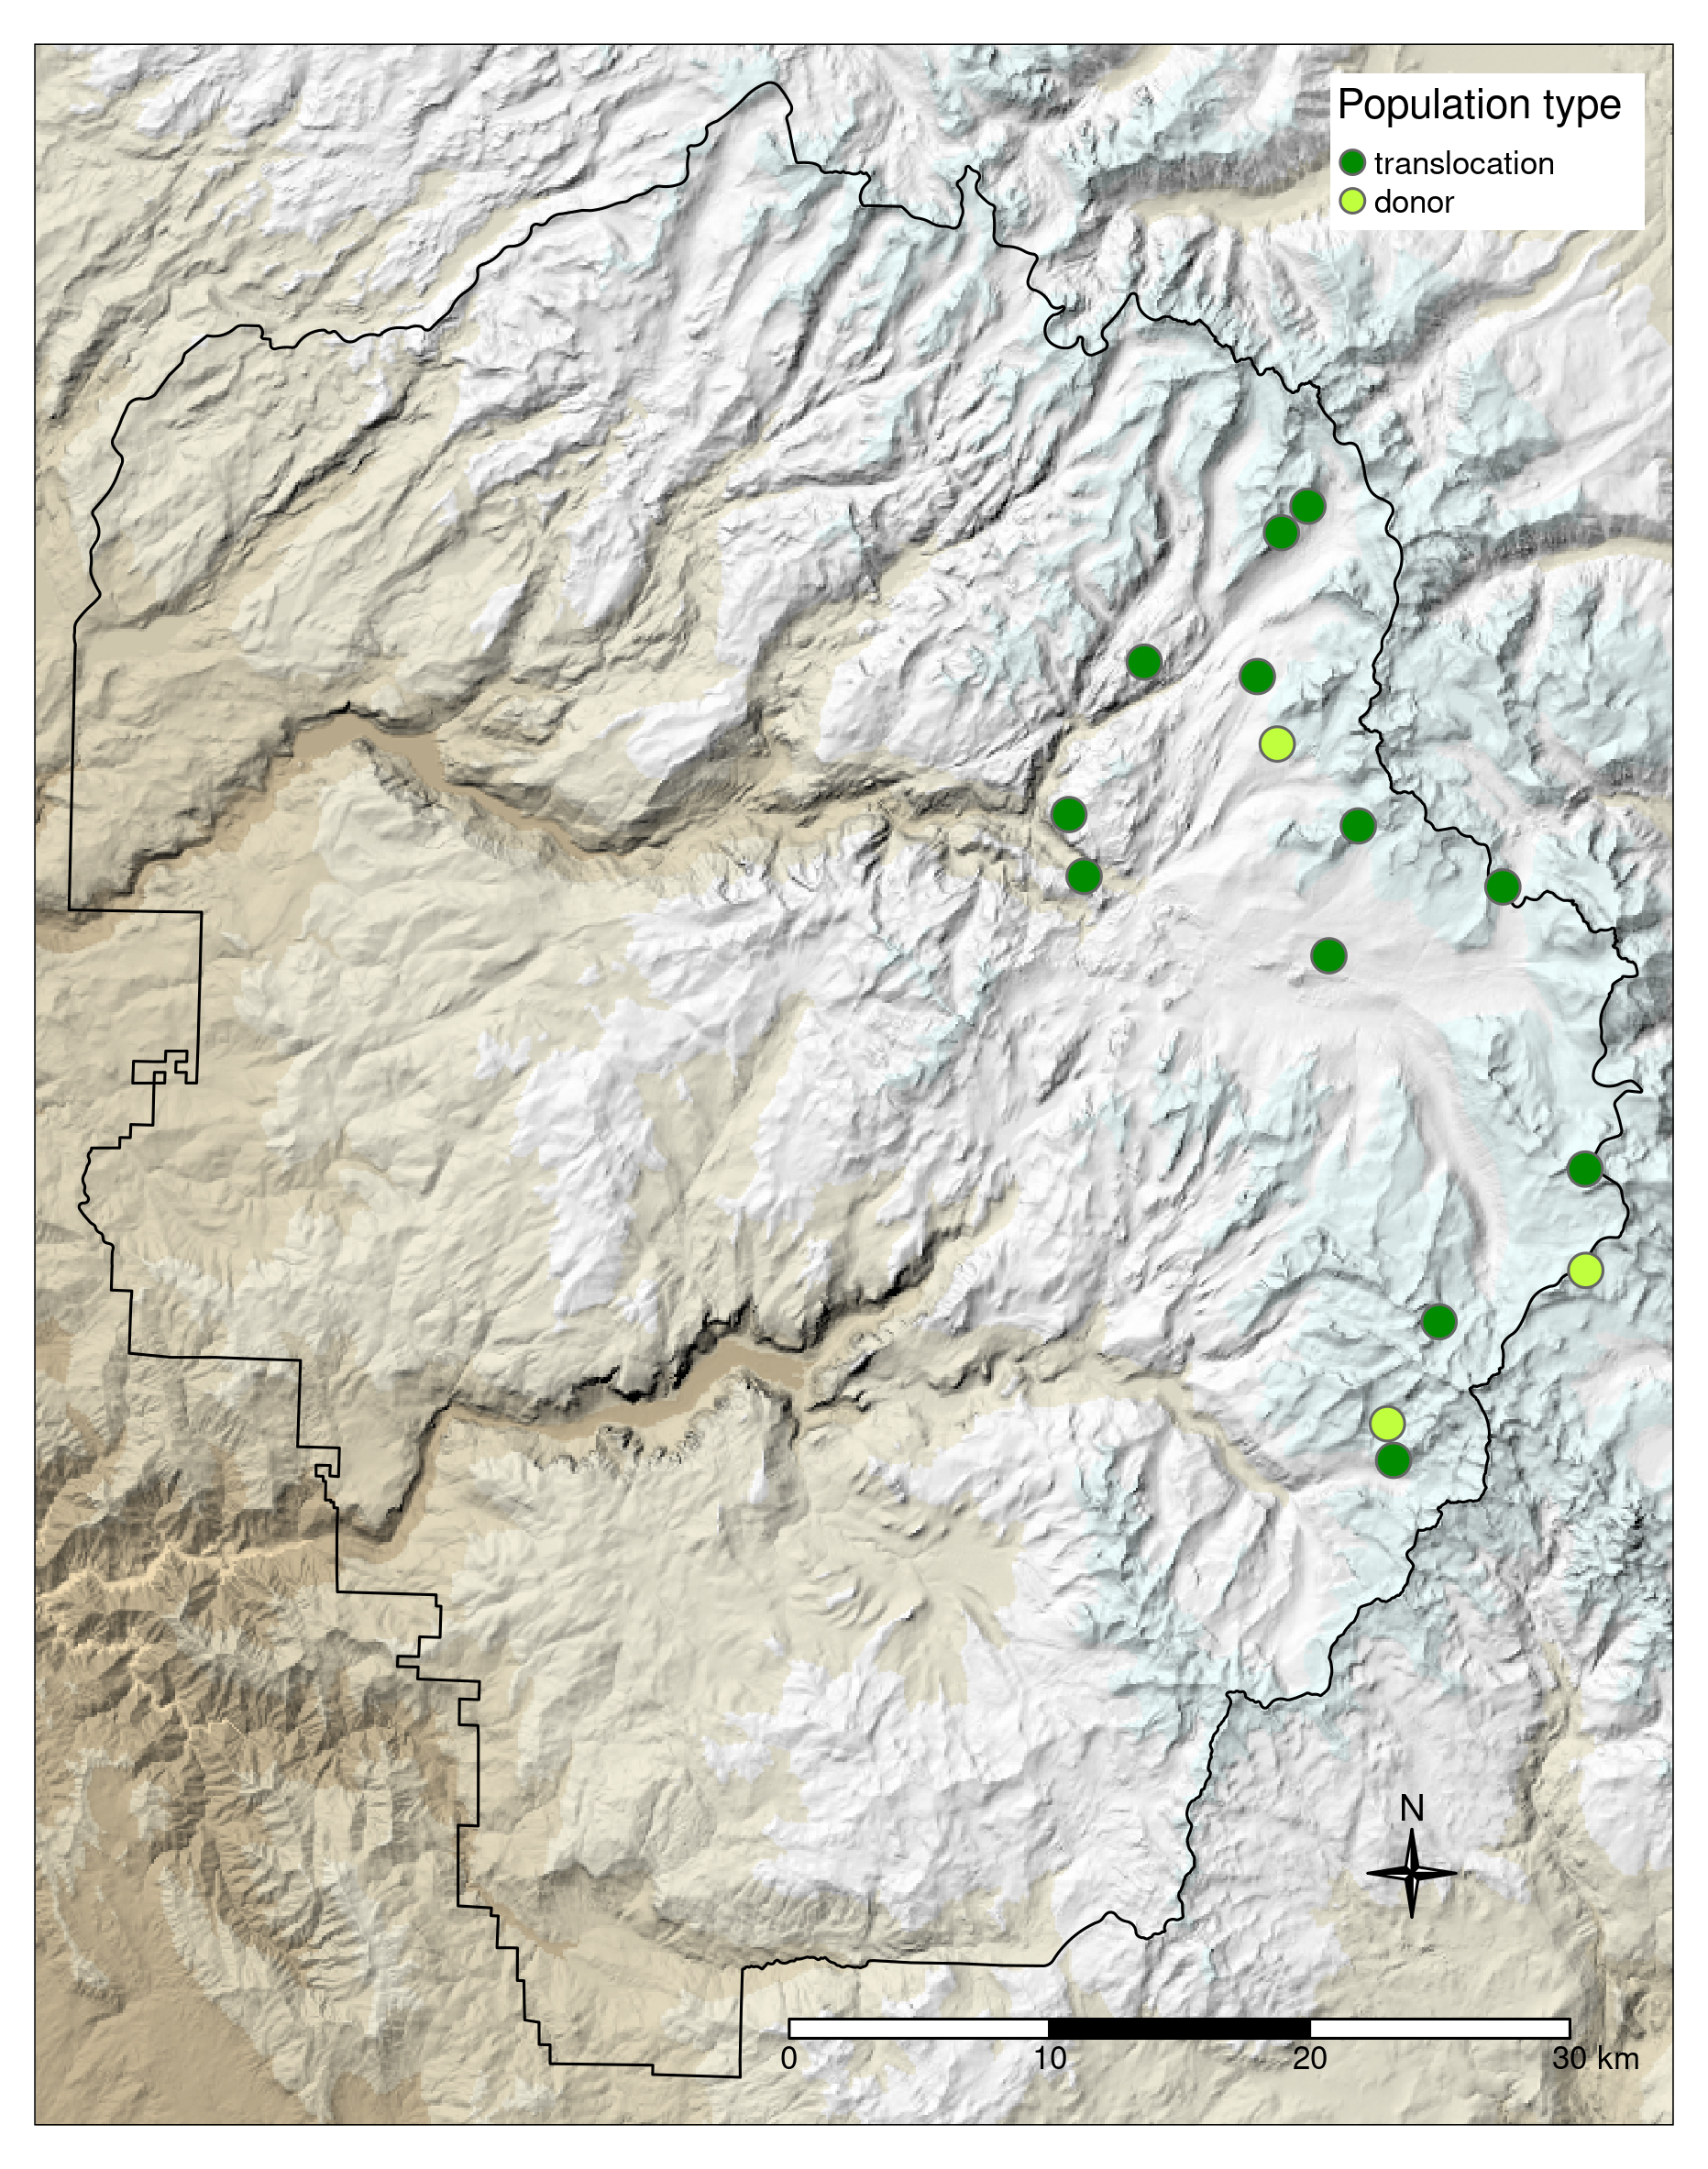
\includegraphics[width=0.60\textwidth]{figures/map_translocation_points.png}

}

\caption{\label{fig-yosemap}Map showing the locations of translocated
and donor MYL frog populations in Yosemite National Park (park boundary
indicated by black polygon). Symbol shapes indicate the donor population
used for each translocation site. To obscure the exact locations of
populations, random noise was added to all point coordinates. Inset map
shows the location of Yosemite within California. In both maps,
elevation is indicated by the colored hillshade layer (dark green =
lowest elevation, white = highest elevation).}

\end{figure}\clearpage

\begin{figure}

{\centering 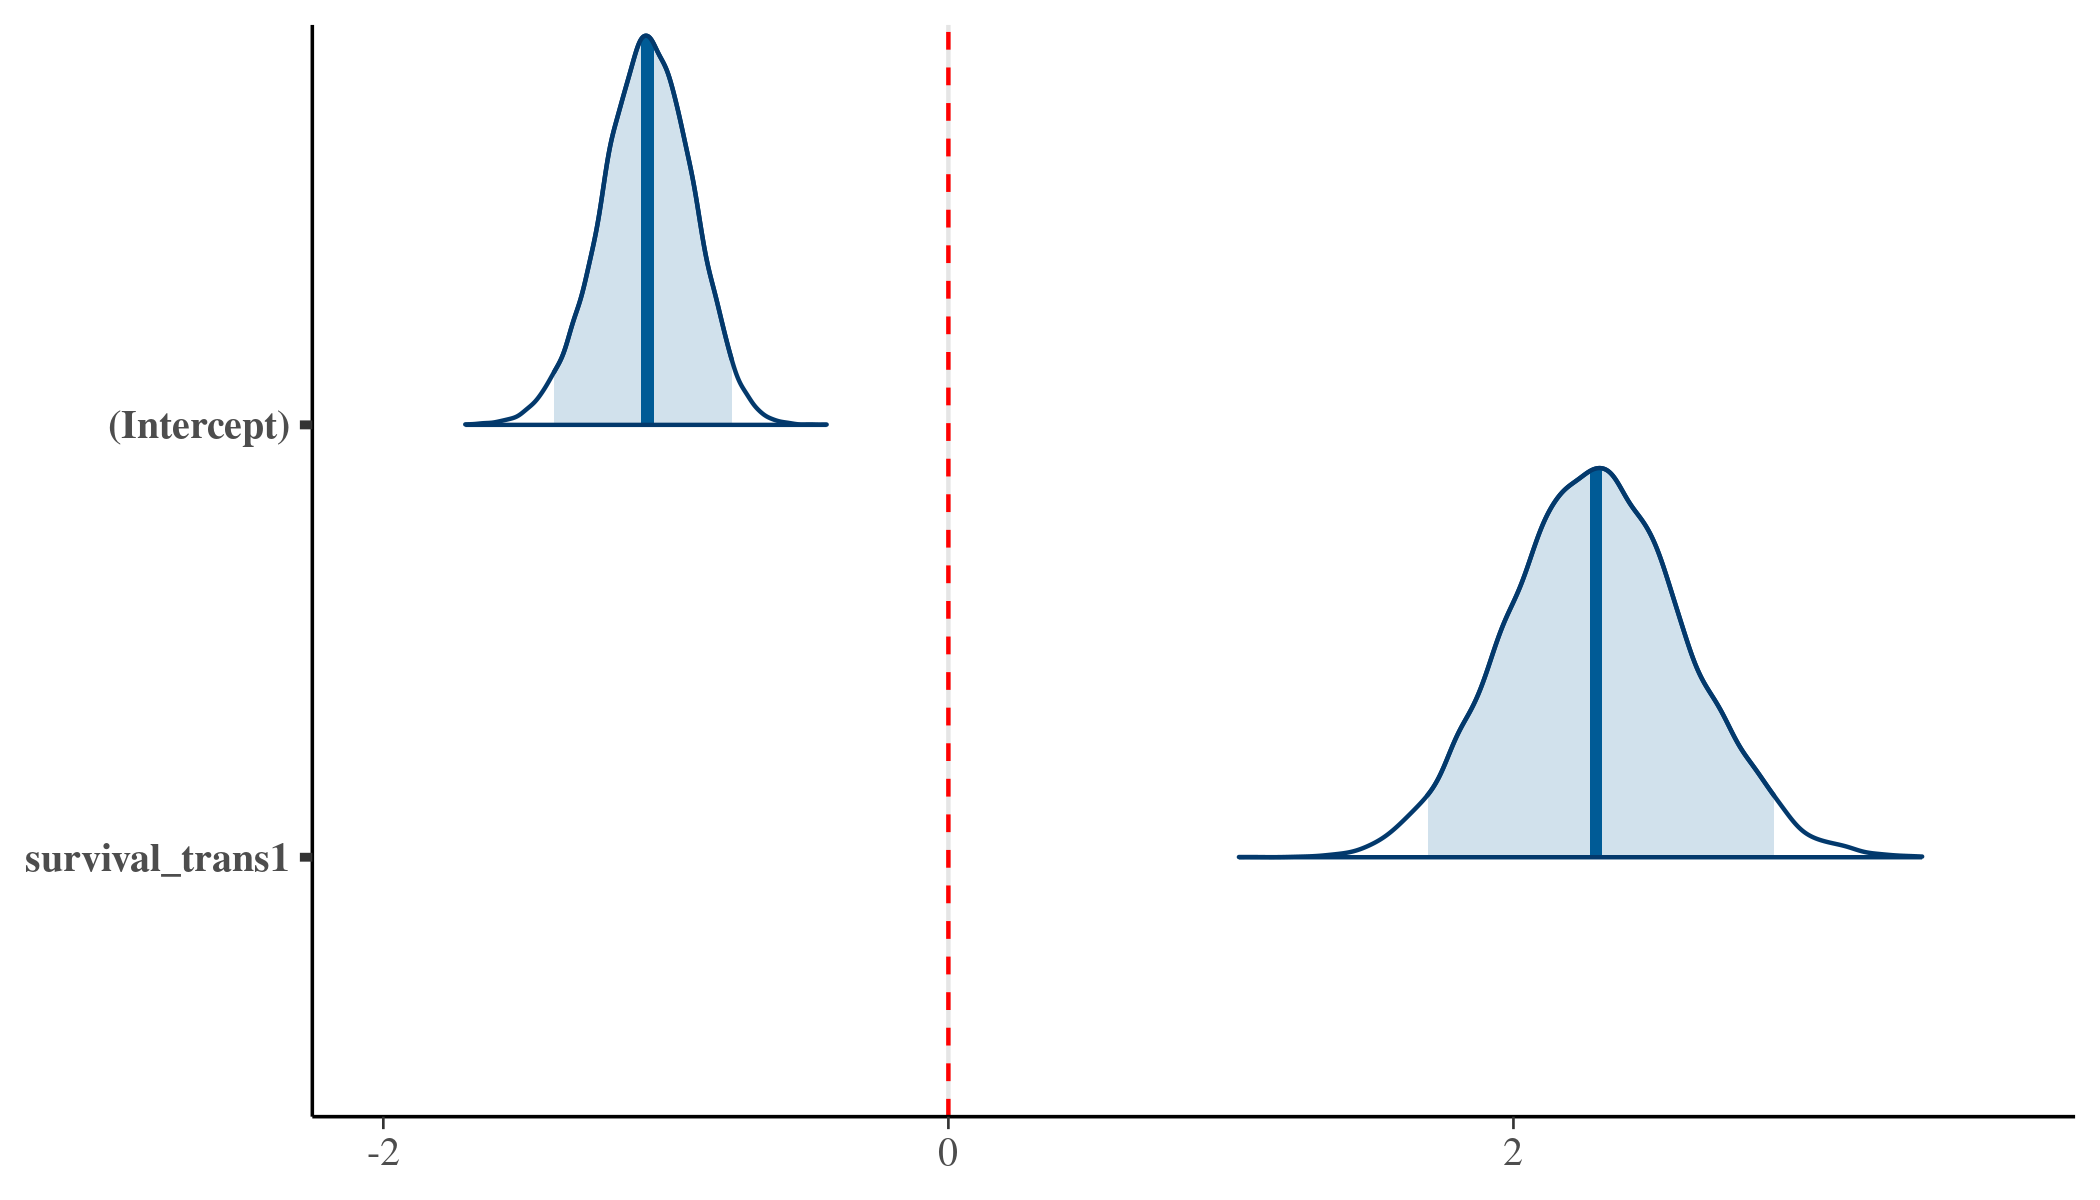
\includegraphics[width=0.60\textwidth]{figures/mcmc_areas_m2b.png}

}

\caption{\label{fig-transsurvival-postdens}For the best model describing
the average 1-year survival of frogs in the first translocation to a
site as a predictor of survival of frogs in all subsequent
translocations to that site, estimated posterior density curves and
shaded 95\% uncertainty intervals for the intercept and single predictor
variable. In the Bayesian framework in which the model was developed, a
variable is considered an important predictor if the associated
uncertainty interval does not overlap zero (indicated by the dashed red
line).}

\end{figure}\clearpage

\begin{figure}

{\centering 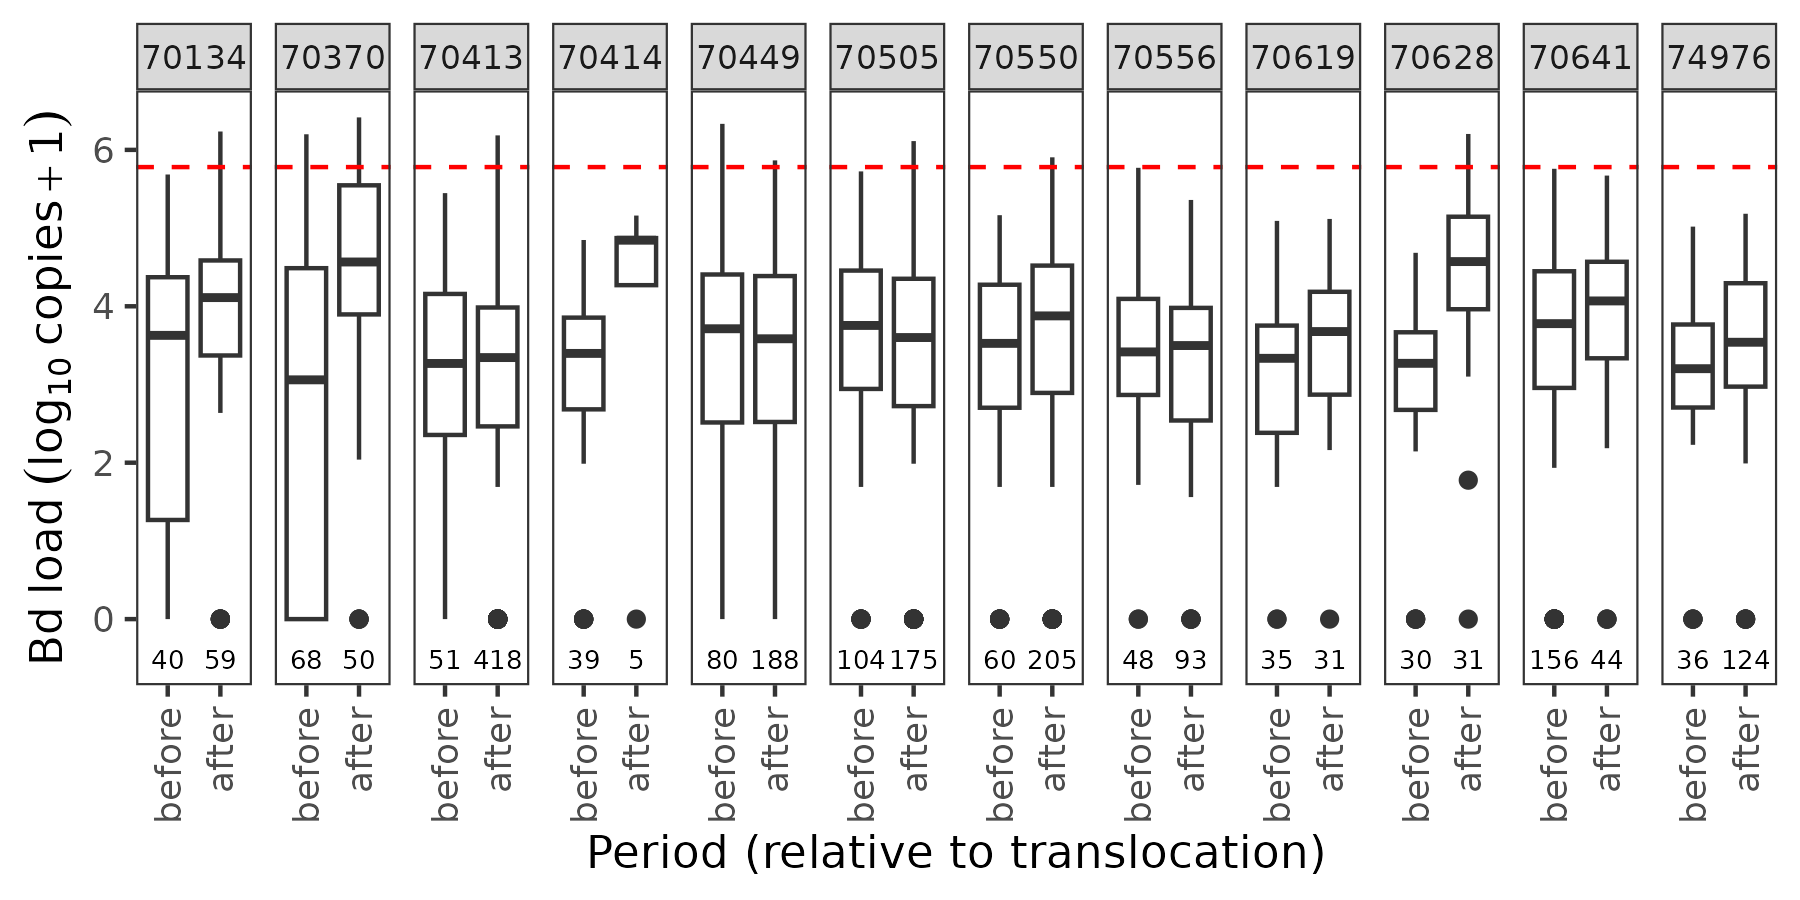
\includegraphics[width=0.7\textwidth]{figures/bdload_beforeafter.png}

}

\caption{\label{fig-bdload-beforeafter}Evidence that frogs translocated
from recovering populations can maintain the benefits of
resistance/tolerance in non-natal habitats. For frogs translocated to
each of the 12 recipient sites, Bd loads for the period immediately
prior to translocation versus during the 1-year period after
translocation. Bd loads are expressed as the number of ITS1 copies per
skin swab, as estimated by qPCR of the Bd ITS1 region. Box plots show
medians, first and third quartiles, largest and smallest values within
1.5x interquartile range, and values outside the 1.5x interquartile
range. Loads indicative of severe disease are \textgreater{} 5.8 ITS
copies (on a log\textsubscript{10} scale).}

\end{figure}\clearpage

\begin{figure}

{\centering 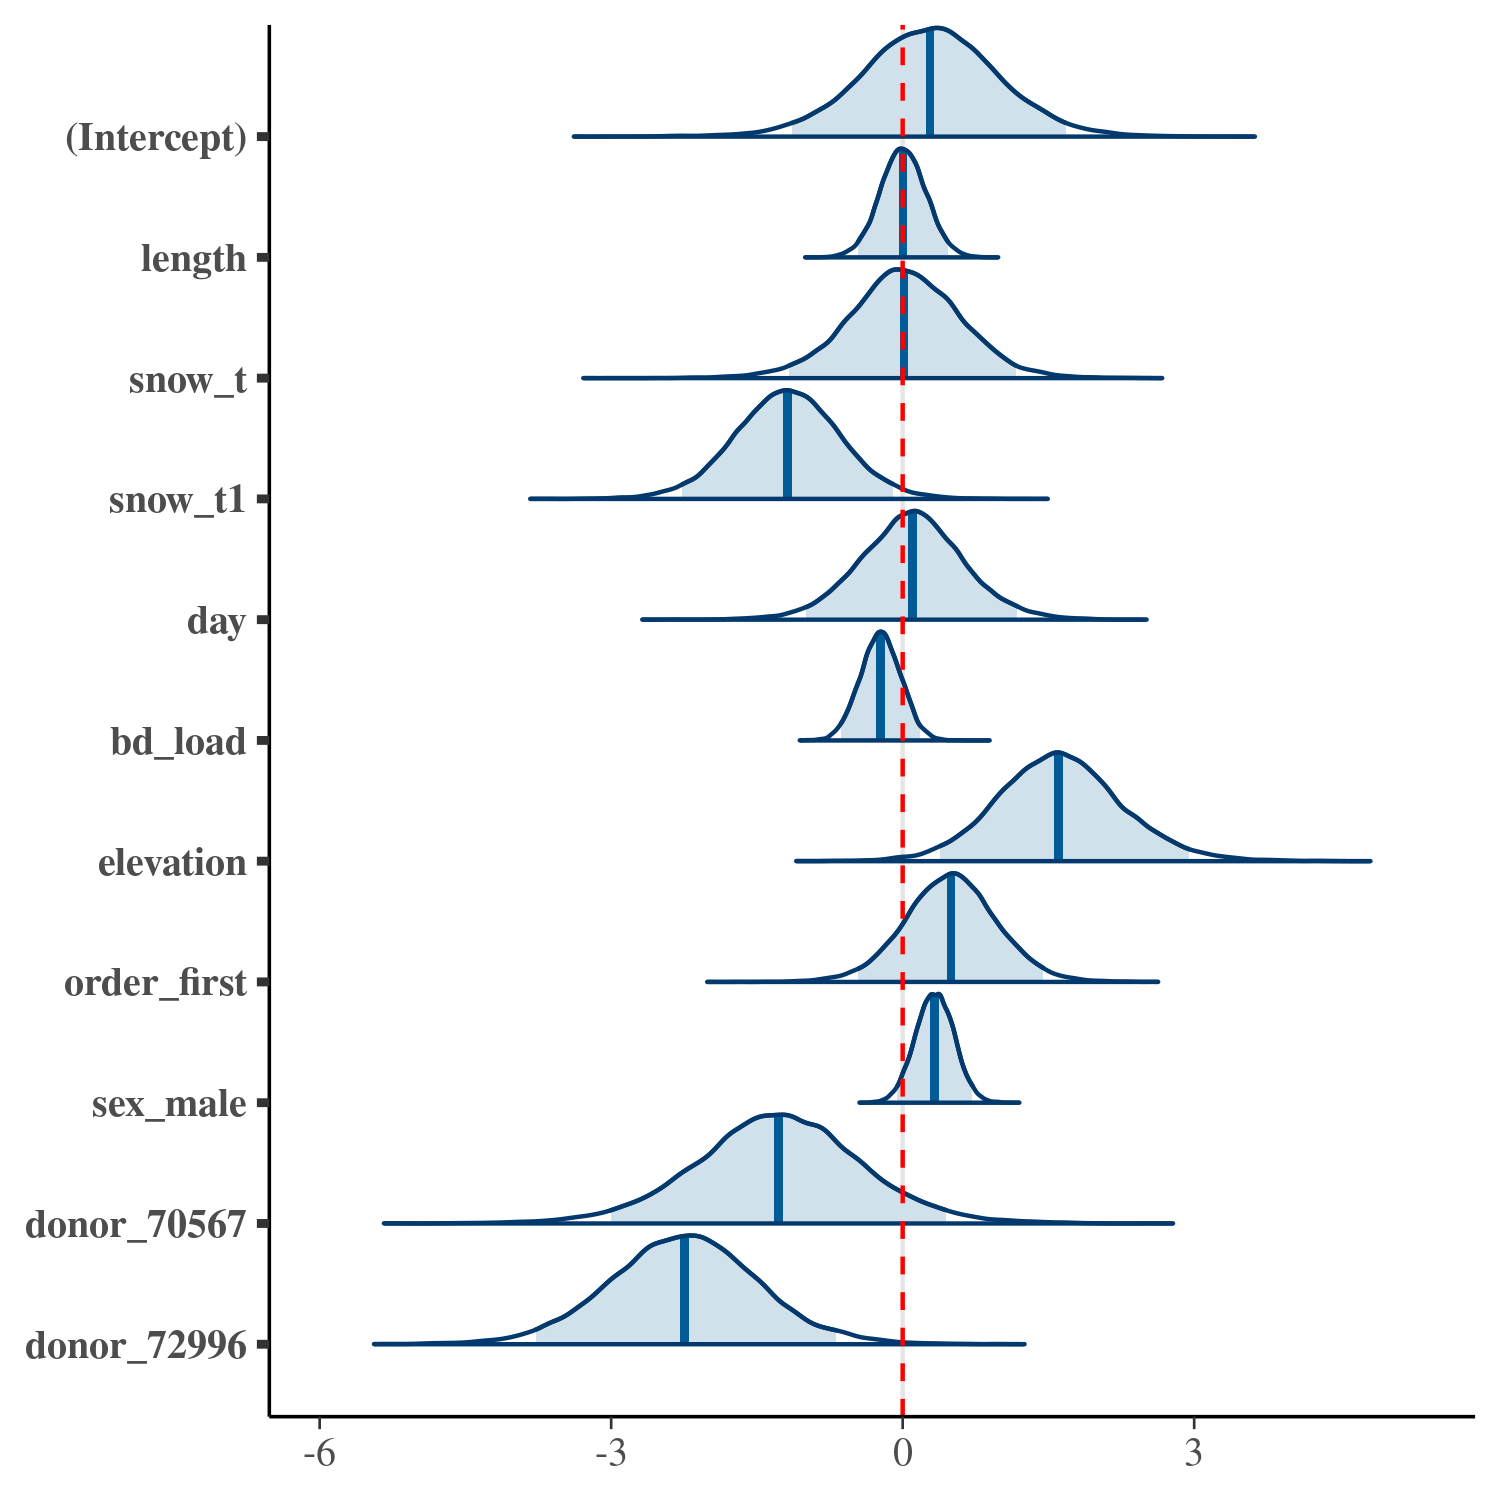
\includegraphics[width=0.60\textwidth]{figures/mcmc_areas_m1d.png}

}

\caption{\label{fig-survival-postdens}Evidence that Bd load is not an
important predictor of post-translocation frog survival. For the best
model identifying predictors of 1-year frog survival following
translocation, estimated posterior density curves and shaded 95\%
uncertainty intervals for the intercept and all predictor variables. In
the Bayesian framework in which the model was developed, variables are
considered important predictors if the associated uncertainty interval
does not overlap zero (indicated by the dashed red line). Predictor
variables shown on the y-axis are defined as follows: length = frog
size, snow\_t = winter severity in the year of translocation (measured
on April 1), snow\_t1 = winter severity in the year following
translocation (measured on April 1), day = day of year on which a
translocation was conducted, bd\_load = Bd load, elevation = site
elevation, order\_first = within-site translocation order, sex\_male =
frog sex, donor\_70567 and donor\_72996 = donor population.}

\end{figure}\clearpage

\begin{figure}

{\centering 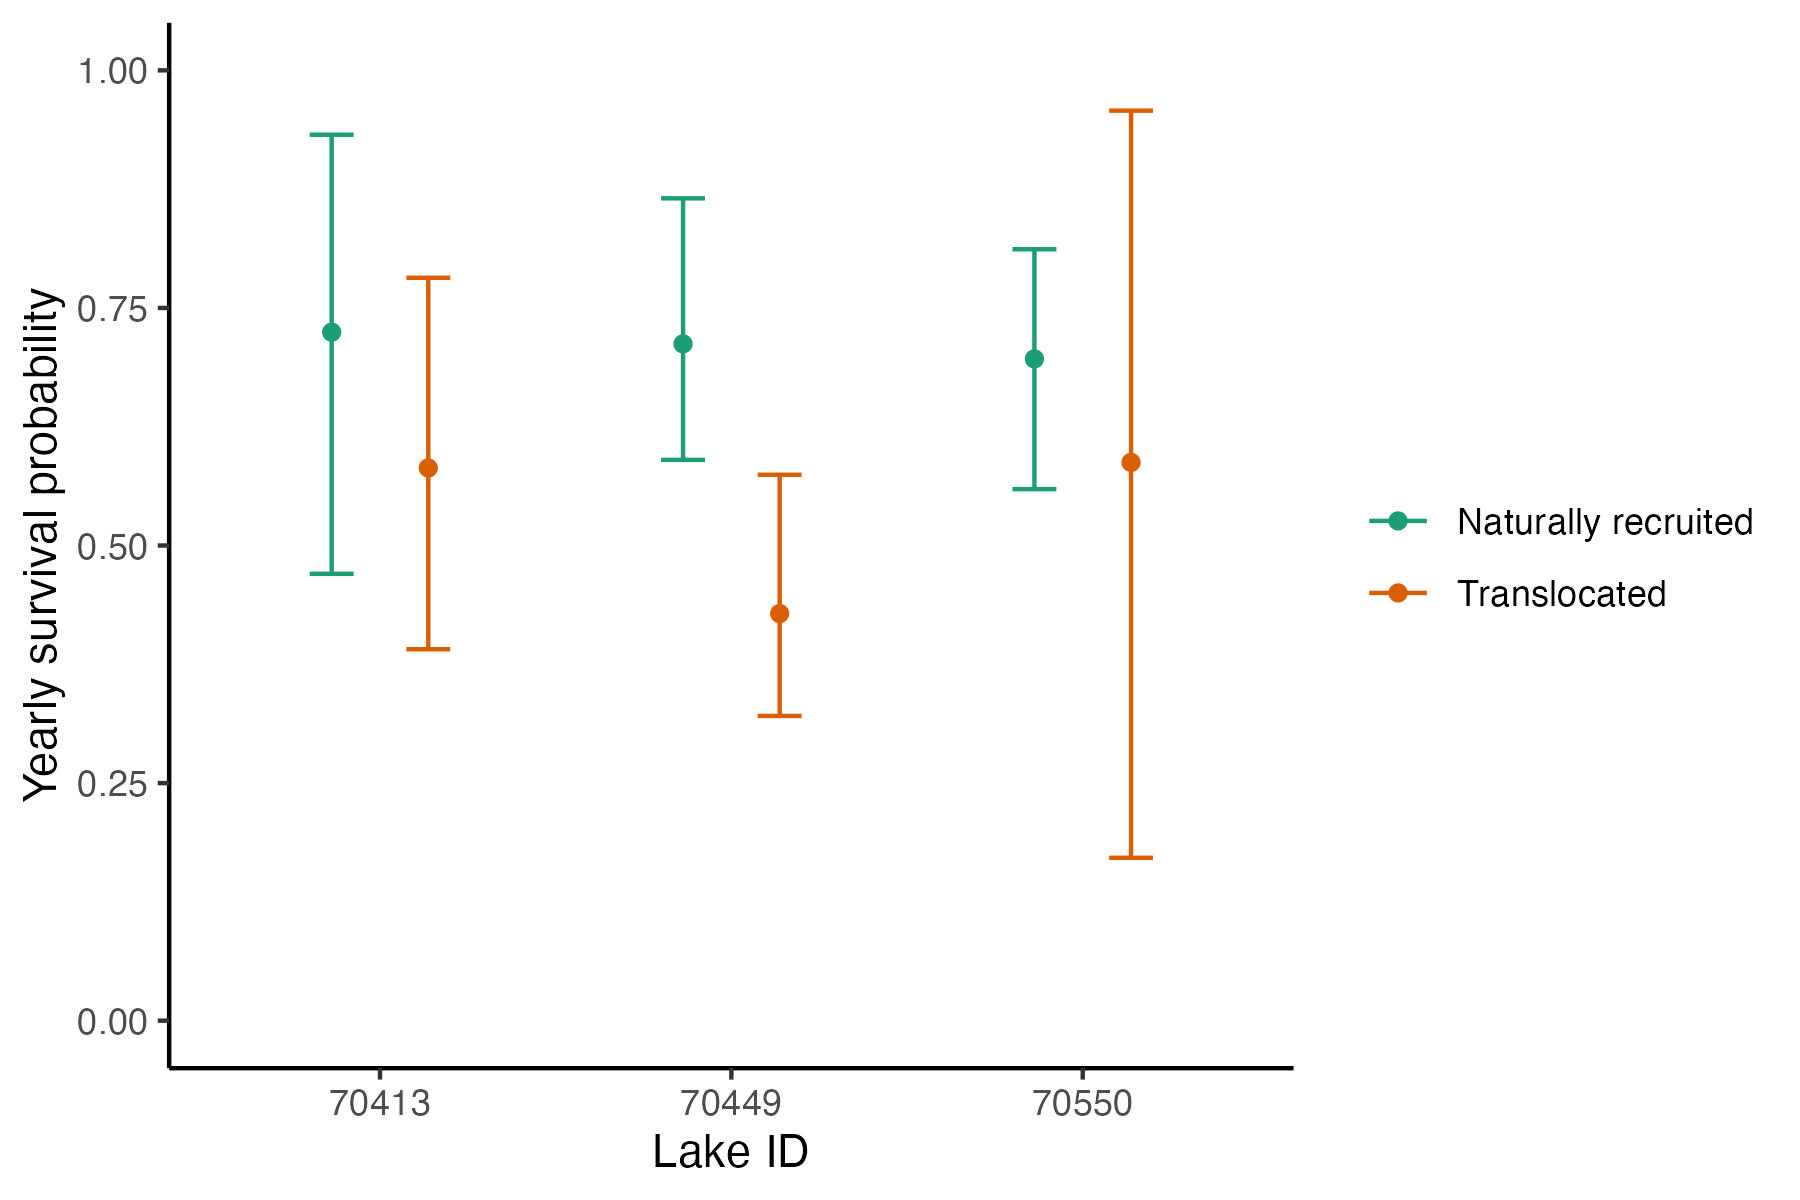
\includegraphics[width=0.60\textwidth]{figures/compare_surv_probs.jpg}

}

\caption{\label{fig-compare_surv_probs}Evidence that frog
resistance/tolerance in non-natal habitats is maintained across
generations. Comparison of the average yearly adult survival
probabilities for adults translocated to each of 3 sites versus adults
that were naturally recruited at each site (as a result of reproduction
by translocated frogs). In contrast to
Fig. 3, these are not survival
probabilities from the first year following translocation, but instead
represent averaged survival probabilities across multiple years and
cohorts. Points are median estimates and error bars give the 95\%
uncertainty intervals around the estimates, accounting for yearly
variation in survival probabilities. All estimates were derived using
the mrmr package.}

\end{figure}\clearpage

\begin{figure}

{\centering 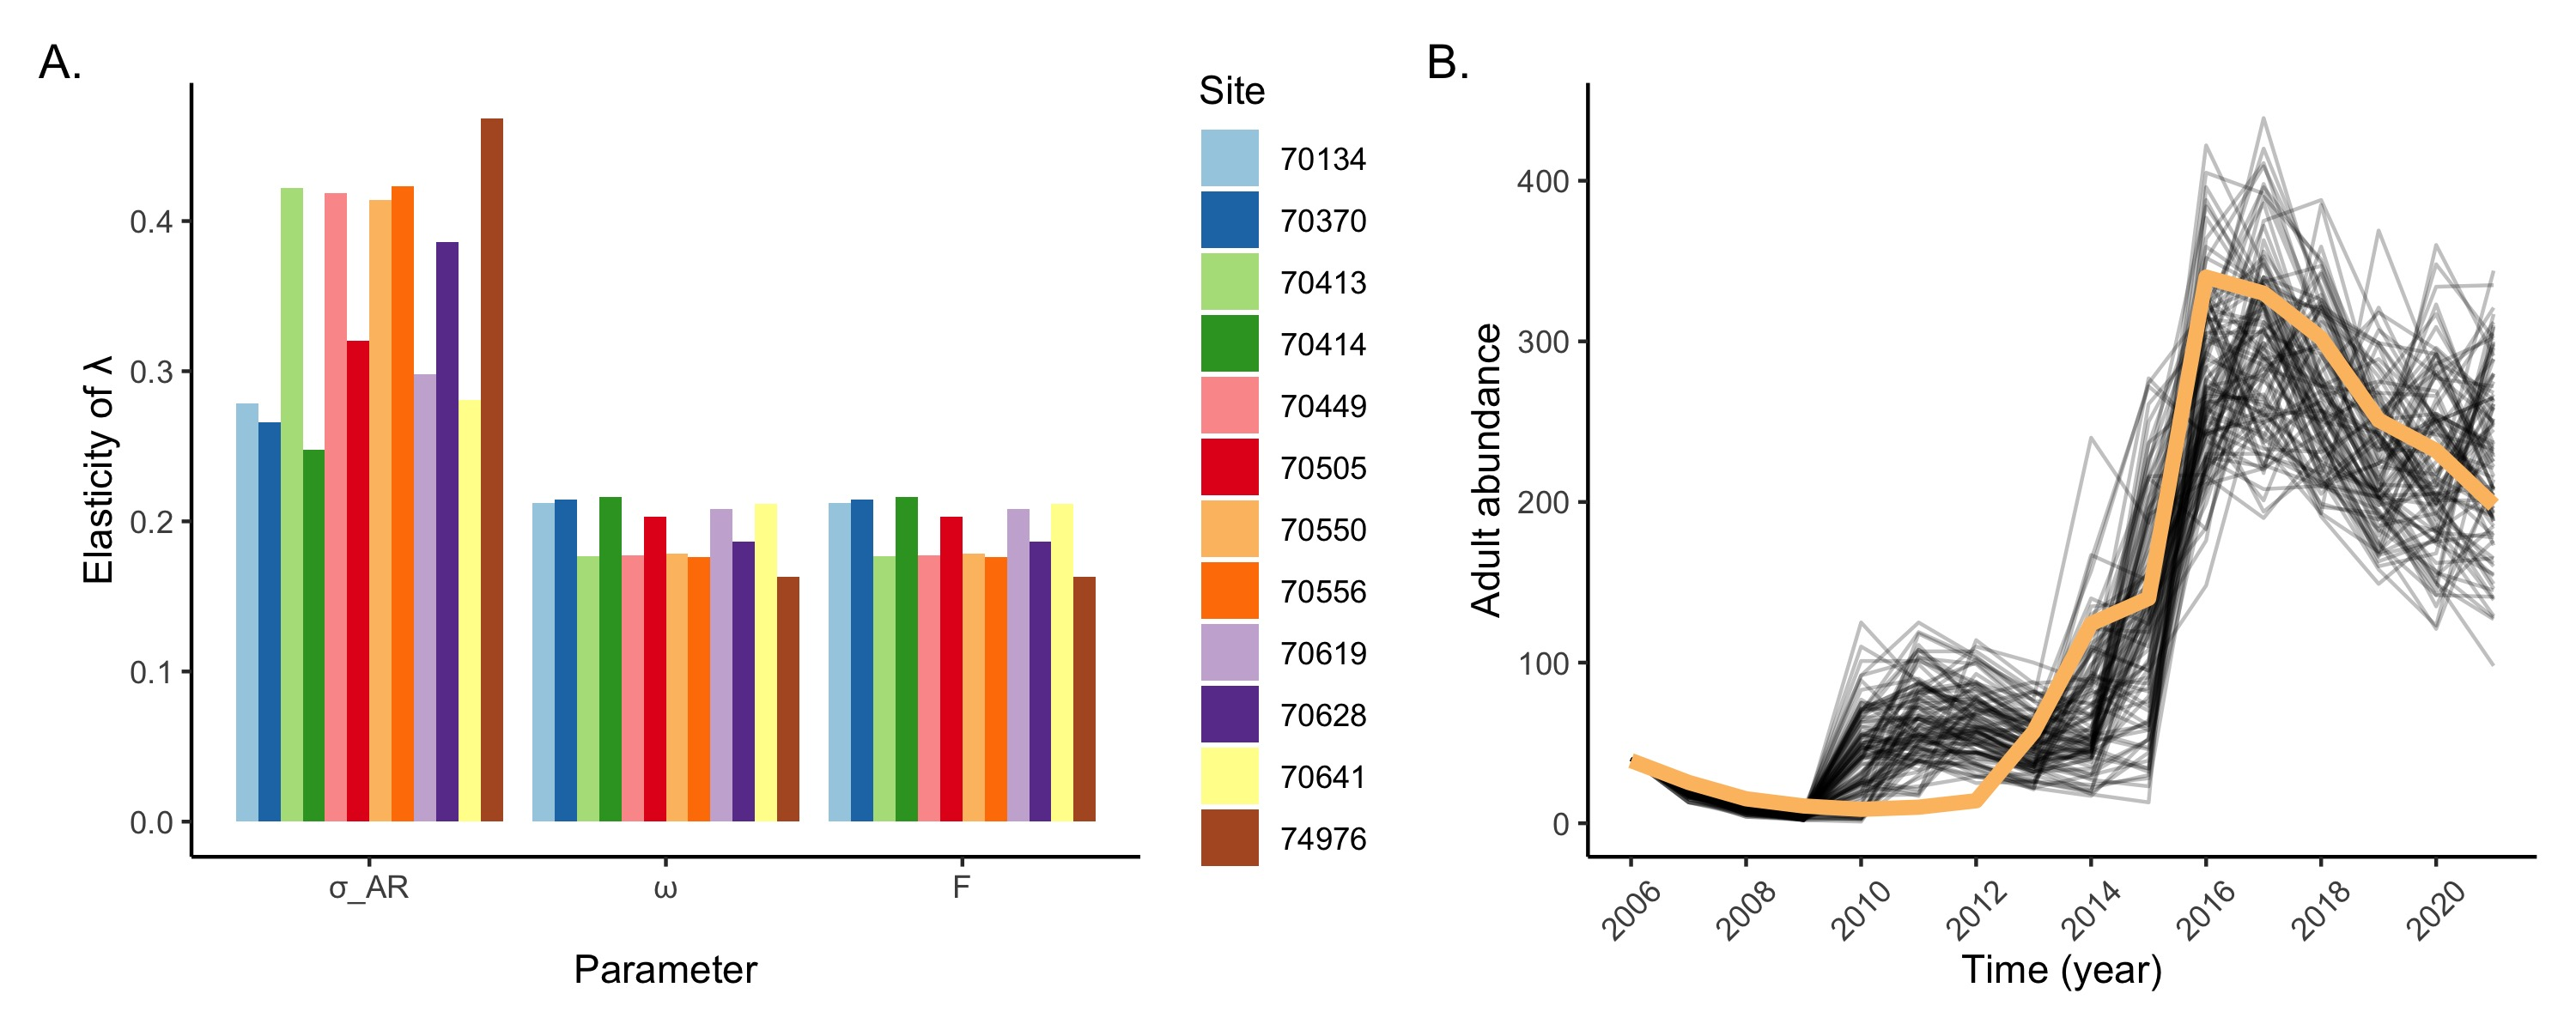
\includegraphics[width=0.60\textwidth]{figures/pop_viability_figures_for_supp.jpg}

}

\caption{\label{fig-viability-supp}Sensitivity analysis of the
stage-structured MYL frog model. Elasticity of \(\lambda\) with changes
in 3 parameters: \(\sigma_{A_R}\) (yearly survival probability of
naturally recruited adults), \(\omega\) (yearly probability of
successful recruitment from juveniles to adults), and \emph{F (}number
of eggs produced by a female frog in a year that successfully hatch).
Elasticity is calculated at the default parameter values for each
population and \(\omega\) = 0.3.}

\end{figure}\clearpage

\newpage

\hypertarget{tables}{%
\subsubsection{Tables}\label{tables}}

\hfill\break



\hypertarget{tbl-survival-earlylate}{}
\begin{longtable}[]{@{}
  >{\raggedright\arraybackslash}p{(\columnwidth - 8\tabcolsep) * \real{0.0654}}
  >{\centering\arraybackslash}p{(\columnwidth - 8\tabcolsep) * \real{0.2056}}
  >{\centering\arraybackslash}p{(\columnwidth - 8\tabcolsep) * \real{0.2430}}
  >{\centering\arraybackslash}p{(\columnwidth - 8\tabcolsep) * \real{0.2056}}
  >{\centering\arraybackslash}p{(\columnwidth - 8\tabcolsep) * \real{0.2804}}@{}}
\caption{\label{tbl-survival-earlylate}Association between the
proportion of populations translocated early versus late in the study
period (\textless{} 2013 or $\geq$ 2013, respectively) and
probability of survival (\textless{} 0.5 or $\geq$ 0.5). Based on
the viability analysis, survival probabilities \textless{} 0.5 and
$\geq$ 0.5 produced 50-year extinction probabilities of 1 and
\textless{} 0.5, respectively.}\tabularnewline
\toprule()
\begin{minipage}[b]{\linewidth}\raggedright
Period
\end{minipage} & \begin{minipage}[b]{\linewidth}\centering
Survival probability
\end{minipage} & \begin{minipage}[b]{\linewidth}\centering
Number of translocations
\end{minipage} & \begin{minipage}[b]{\linewidth}\centering
Total translocations
\end{minipage} & \begin{minipage}[b]{\linewidth}\centering
Proportion of translocations
\end{minipage} \\
\midrule()
\endfirsthead
\toprule()
\begin{minipage}[b]{\linewidth}\raggedright
Period
\end{minipage} & \begin{minipage}[b]{\linewidth}\centering
Survival probability
\end{minipage} & \begin{minipage}[b]{\linewidth}\centering
Number of translocations
\end{minipage} & \begin{minipage}[b]{\linewidth}\centering
Total translocations
\end{minipage} & \begin{minipage}[b]{\linewidth}\centering
Proportion of translocations
\end{minipage} \\
\midrule()
\endhead
early & \textless{} 0.5 & 4 & 5 & 0.800 \\
early & $\geq$ 0.5 & 1 & 5 & 0.200 \\
late & \textless{} 0.5 & 2 & 7 & 0.286 \\
late & $\geq$ 0.5 & 5 & 7 & 0.714 \\
\bottomrule()
\end{longtable}

\newpage

\hypertarget{tbl-param_values}{}
\begin{longtable}[]{@{}
  >{\raggedright\arraybackslash}p{(\columnwidth - 4\tabcolsep) * \real{0.3750}}
  >{\raggedright\arraybackslash}p{(\columnwidth - 4\tabcolsep) * \real{0.2639}}
  >{\raggedright\arraybackslash}p{(\columnwidth - 4\tabcolsep) * \real{0.3611}}@{}}
\caption{\label{tbl-param_values}Description and values of parameters
used in the model. All survival probabilities are in the presence of the
fungal pathogen Bd.}\tabularnewline
\toprule()
\begin{minipage}[b]{\linewidth}\raggedright
\textbf{Parameter}
\end{minipage} & \begin{minipage}[b]{\linewidth}\raggedright
\textbf{Value}
\end{minipage} & \begin{minipage}[b]{\linewidth}\raggedright
\textbf{Source}
\end{minipage} \\
\midrule()
\endfirsthead
\toprule()
\begin{minipage}[b]{\linewidth}\raggedright
\textbf{Parameter}
\end{minipage} & \begin{minipage}[b]{\linewidth}\raggedright
\textbf{Value}
\end{minipage} & \begin{minipage}[b]{\linewidth}\raggedright
\textbf{Source}
\end{minipage} \\
\midrule()
\endhead
\(\sigma_{L_1}\), Yearly survival probability of year 1 tadpoles & 0.7 &
Estimated from field data, observations, natural history knowledge \\
\(\sigma_{L_2}\), Yearly survival probability of year 2 tadpoles & 0.7 &
Estimated from field data, observations, natural history knowledge \\
\(\sigma_{L_3}\), Yearly survival probability of year 3 tadpoles & 0.7 &
Estimated from field data, observations, natural history knowledge \\
\(\sigma_{J_1}\), Yearly survival probability of year 1 juveniles & 0.25
& Estimated from field data, observations, natural history knowledge \\
\(\sigma_{J_2}\), Yearly survival probability of year 2 juveniles & 0.5
& Estimated from field data, observations, natural history knowledge \\
\(\sigma_{A_R}\), Yearly survival probability of naturally recruited
adults & Varies by population & Estimated from mark-recapture studies \\
\(\sigma_{A_T}\), Yearly survival probability of translocated adults &
Varies by population & Estimated from mark-recapture studies \\
\(p_{L_1}\), Probability of a year 1 tadpoles remaining as a tadpoles &
1 & Estimated from field data, observations, natural history
knowledge \\
\(p_{L_2}\), Probability of a year 2 tadpoles remaining as a tadpoles &
0.25 & Estimated from field data, observations, natural history
knowledge \\
\(p_{J_1}\), Probability of a year 1 juvenile remaining as a juvenile &
0.25 & Estimated from field data, observations, natural history
knowledge \\
\(p_F\), Probability of a adult female reproducing in a year & 0.5 &
Could be as high at 1, based on field observations \\
\(F\), Number of surviving eggs produced by an adult female & 100 & From
observations of captive frogs \\
\(\omega\), Probability of juvenile successfully recruiting to an adult
& Varies yearly & Explored different values of this parameter \\
\bottomrule()
\end{longtable}

\newpage


%%% Add this line AFTER all your figures and tables
\FloatBarrier

\dataset{gemma\_outliers\_all.csv}{Set of liberal SNP and INDEL outlier variants (Bonferroni corrected p-value $<$ 0.05), identified via GEMMA.}

\dataset{gemma\_outliers\_strict\_freq.csv}{Set of strict SNP and INDEL outlier variants (Bonferroni corrected p-value $<$ 0.01), identified via GEMMA.
Additional information includes variant location within the gene (predicted\_gene\_loc) and whether the variant is synonymous or nonsynonymous (predicted\_effect\_AA).}

\dataset{spline\_window\_shared\_outliers.csv}{Description of overlapping \emph{F\textsubscript{ST}} and
\(\pi_{diff}\) outlier windows, as identified in the splined window
analysis.}

\dataset{spline\_window\_gene\_details.csv}{Annotation information for all genes within each of the
overlapping outlier windows in dataset S3}

\bibliography{translocation}

\end{document}

